\setchapterpreamble[u]%{\dictum[Larry Wall]{I don't know\\if it's what you want,\\but it's what you get. :-)}}

\chapter{Realization} \label{chap:Realization}
\minitoc\vspace{1em}

The problem is realized as a two part solution using the Client-Server architecture.


\section{Background}

\subsubsection{Java Technology}
The implementation of this project is done using Java \todo{Java Cite}{How to cite technologies?}.
Java technology refers to both the programming language and the platform.
The Java programming language is high level object oriented language\cite{Gosling:2014:JLS:2636997}, 
which is actively developed and supported. 
The Java Software Platform provides a system for developing application software and deploying it in a cross-platform computing environment. 
There are several Java platforms.
The Enterprise Edition (Java EE) platform provides an API and runtime environment for developing and running enterprise software, such as web services.

\subsubsection{JGraphT}

JGraphT is an open-source Java library specialized for graph-theory modelling and algorithms.It suppoerts several different types of graphs\cite{JGraphT}:
\begin{itemize}
	\item[--] Directed and undirected graphs
	\item[--] Graphs with labeled, unlabeled, weighted or unweighted edges
	\item[--] Edge multiplicity (more than one edge between two vertices)
	\item[--] Composition of all above
\end{itemize}

The JGraphT API implements vast number of important algorithms, such as PageRank, Random Walk, graph analysis, centrality etc.
JGraphT also provides an integration with the JGraph\footnote{\url{https://jgraph.com/}} library for elementary graph visualization.

\subsection{GraphStream}

GraphStream is a Java library for the modeling and analysis of dynamic graphs\cite{GraphStream}. 
It is distributed in three packages: \emph{gs-core} - for the basic graph creation, 
\emph{gs-algo} - algorithms that are run on a graph  and
\emph{gs-ui} that contain contain sources for graphical tools.
Besides generating and measurement of graphs, it offers API for simple visualizations. 

\subsubsection{Gephi}

Gephi - The Open Graph Viz Platform is a open-source graph analysis tool, 
which provides rich visualizations and advanced exploration\cite{Gephi}.
The graphs can be of directed, undirected or mixed type\cite{Gephi:GraphAPI}.
Gephi offers filtering of the graphs by using attributes or built-in properties, 
such as in-degree to get more compact representation of the graph. 
It also supports determining modularity, centrality, detecting communities and similar layering algorithms.
Gephi is realized as a third-party tools, intended for non specialists i.e\. easy to use.

\subsubsection{R}

R is a language and environment for statistical computing and graphics\cite{R-project}.
It provides support for machine learning techniques and data analysis (classification, regression, time series analysis etc.).
The extension of the functionalities of R is done through packages.
The main repository Cran\footnote{\url{https://cran.r-project.org/web/packages}} 
contains 9833 packages as the time of writing (January 2017).

\section{Data Analysis Stages} \label{sec:steps}
According to \cite{Ojeda:2014:PDS:2721420}, we divided the analysis in five stages (Figure\ref{fig:datasteps}):
\begin{enumerate}
	\item \textbf{Data acquisition and importing}: 
	The first step in the pipeline is to acquiring the data and import it into our system. 
	The data can come from different sources and can exist in various formats.
	\item \textbf{Data wrangling and manipulation}: 
	Data is rarely in the desired format. 
	This step includes transforming and bringing the data in more convenient format.
	The purpose is to allow easy consumption for analysis.
	\item \textbf{Exploratory Analysis}: 
	The third step is to come to an understanding of the data that will be used. 
	This includes steps like visualization, summarization of characteristics, counting etc.
	\item \textbf{Modeling and analysis}: 
	This step is the core of the work. 
	Here we build and test various models for similarity, clustering and other machine learning use-cases.
	\item \textbf{Integrating and operationalizing}: 
	At the end of the pipeline we need to make use of the data back in a compelling form and structure,
	both for ourselves and as a response for API requests. 
\end{enumerate}

\begin{figure}[ht]
	\centering
	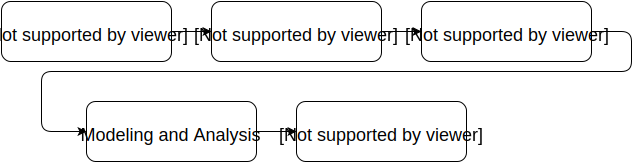
\includegraphics[width=0.7\textwidth]{data_steps.png}
	\caption{The work--flow of the data analysis} 
	\label{fig:datasteps}
\end{figure}

\section{Server Side}
The steps listed in \ref{sec:steps} are implemented on the server side.
\subsubsection{Data Acquisition}
The data was provided from a company, consisting of two main data sources: 
the repository data and the Architecture model project data.

The repository is obtained from the Abacus in XML format. It is composed from the following parts:
 \begin{itemize}
 	\item[--] Shapes: contains geometric and visual information for the components, such as position, color, gradient etc.
 	\item[--] Standards: \todo{explain}{To what do the Standards correspond?}
 	\item[--] Types: Contains the possible types of the components and the connections
 	\item[--] Templates: \todo{explain}{To what do the Templates correspond?}
 	\item[--] Architecture: Contains all the components and the connections between them
\end{itemize}

The architecture projects files are also in XML format. 
They are exported from the \emph{Archi} modelling tool. 
The structure is organized into two main attributes: “Folders” and “Properties”. 
The Folders correspond the ArchiMate architecture layers (Business, Application, Technology, Motivation and Implementation \& Migration), plus two additional folders:
\begin{itemize}
		\item[--] Relations: information about all the connections between components
		\item[--] Views: the user-defined alongside with the components and relations that are specific for that view		
\end{itemize}
Alternatively, the project files can also be exported to CSV format. In this case, there are three generated CSV files: Components, Relations and Properties.

\textbf{Parsing XML into Java Objects}: 
The parsing of the repository XML data and the project files is done using the Java DOM Parser.
For the repository, we are interested in the content of the \emph{Architecture} section 
(where the components and the connections are kept) and the \emph{Types} section 
(where the type of every component and connection is stored).
The DOM defines several Java interfaces, of which most important are elements and their attributes. 
The \emph{Component} and the \emph{Relation} elements are parsed into Java objects \emph{Component} and \emph{Connection} respectively, with properties that reflect the element attributes.

\todo{Figure}{The Object Diagram of Component and Connection}

\subsubsection{Data Wrangling}
After successfully importing the data, we decide on the features to use, and how to model the data. 
For analysis purposes, we use the $name$, the $type$ and $description$ properties of the components. 
\textbf{Graph Representation}:
For modeling the interaction between components via relations, we use the \emph{JGraphT} library. 
The chosen graph model is the \emph{DirectedGraph}, which is parametrized for the node and edge type. 
It provides direct interfaces for adding nodes and edges. 
Prerequisite for adding the edges is that both of the nodes (the source and the sink) should be added in the graph beforehand.

\begin{lstlistingJava}{}
		import org.jgrapht.graph.DefaultDirectedGraph;
		import org.jgrapht.DirectedGraph;
		
		/* Directed graph using Component as nodes 
		and Connection as edges*/
		DirectedGraph<Component, Connection> graph 
			= new DefaultDirectedGraph(Connection.class);
\end{lstlistingJava}

\subsubsection{Exploratory Analysis}
To get basic understanding of the components from the repository and their interaction, a visualization of the graph is needed. 
For the very impression, we used the $GraphStream$. 
First step was providing different graph model and :
\begin{lstlistingJava}{}
		import org.graphstream.graph.Graph;
		import org.graphstream.graph.implementations.MultiGraph;
		
		Graph graph = new MultiGraph("Repository");
		addNodes(graph, abacus.getComponents());
		addEdges(graph, abacus.getConnections());
		display(graph);
\end{lstlistingJava}
GraphStream automatically repositions the nodes within a graph to find the most suitable spacing.
As achieving stability is a time consuming step, we provide the visualization after interval of 5 seconds\ref{fig:graphstream}.
\begin{figure}[ht]
	\centering
	\includegraphics[width=0.7\textwidth]{screenshotGraphstream.png}
	\caption{Visualization of the repository using \emph{GraphStream}} 
	\label{fig:graphstream}
\end{figure} 

The total size of the repository data is 3922 nodes with 9657 edges.
%2775 are connected
\section{Client Side}